\documentclass[../main/report.tex]{subfiles}
\begin{document}

\chapter{NVIDIA's Fermi Architecture and CUDA Programming Model}
\label{sec:fermi}

%http://www.nvidia.com/content/PDF/fermi_white_papers/P.Glaskowsky_NVIDIAFermi-TheFirstCompleteGPUComputingArchitecture.pdf
%http://www.nvidia.com/content/PDF/fermi_white_papers/NVIDIA_Fermi_Compute_Architecture_Whitepaper.pdf

To explore some concepts of modern GPU architectures in detail, this chapter will take a look at an example from NVIDIA.
The programming model used by NVIDIA for its modern GPUs, called CUDA, will be be examined.
Then, NVIDIA's first architecture to use this programming model, the Fermi architecture, will be used as the example for illustrating GPU design concepts.  
Demolicious is heavily inspired by NVIDIA, and the following concepts are relevant for both its programming model and its architecture.


\section{The Fermi Architecture}

In 2006 NVIDIA released their first GPUs with a so called \emph{unified shader architecture}.
Before this, GPUs had separate, dedicated hardware for all common graphics operations. 
Beginning with the Fermi architecture, the majority of operations are executed on the same hardware.
The hardware is able to perform general operations.
This significant difference compared to earlier GPU microarchitectures has enabled other calculations on a GPU than graphics processing.
This ability been given the term General-Purpose GPU computing, or GPGPU.


\section{CUDA Programming Model}
\label{sec:cuda_prog_model}

To open up the computing powers of the graphics card for general applications, there was a need for a new application programming interface (API) that could be used run code on the GPUs.
It was possible to do non-graphical calculations on GPUs previously, but it required redefining any problem as a graphical problem.
This was highly impractical. 
With the Fermi architecture, NVIDIA released a framework for running code on their GPUs called CUDA.

CUDA is an extension to the programming language C, and it lets the programmer write functions for executing on the GPU.
Such a function is called a \emph{kernel}.
An example will be used to illustrate how a kernel executes on the Fermi architecture.

Let's say you want to fill a frame buffer, an area of memory, with the color green.
We'll assume that the memory area starts at location 0.
In a sequential programming model, you would typically write a loop that would fill
the memory locations with the value for green one by one.
See Listing \ref{lst:sequential-green}.

\begin{c-code}[caption=A sequential program filling the screen with green, label=lst:sequential-green]
int green = 0x00FF00;
for (int i = 0; i < nr_of_pixels; i++){
	framebuffer[i] = green;
}
\end{c-code}

For a CUDA kernel, on the other hand, the loop would be written as if filling only a single pixel with green. 
The kernel would then be executed by one thread for every pixel in the screen.
Each thread would receive a unique id number corresponding to the 'i' value from the serial example.
Below, in Listing \ref{lst:cuda-green-kernel}, is an example CUDA kernel that fills a single memory location, or pixel, with green.

\begin{c-code}[caption=A CUDA kernel filling a single pixel with green, label=lst:cuda-green-kernel]
__global__ void fill_screen(int* framebuffer){
	/* Calculate global id of this thread */
	int global_id = blockIdx.x * blockDim.x + threadIdx.x; 
	int green     = 0x00FF00;
	framebuffer[global_id] = green;
}
\end{c-code}

The CPU will need to load a kernel into the GPU at run time before calling it.
When calling a kernel, the CPU specifies how many threads to run for it.
Managing memory on the GPU and uploading and calling kernels on it is done using CUDA specific syntax.
Listing \ref{cuda-kernel-launch} shows example CUDA code for calling the "fill\_screen" kernel.

\begin{c-code}[caption=Starting the CUDA kernel with one thread per pixel on a 1920x1080 screen, label=cuda-kernel-launch]
int* frame_buffer_device = cudaMalloc(@); // allocate memory at GPU
fill_screen<<<1080,1920>>>(frame_buffer_device); // call kernel
\end{c-code}

Running a separate thread for each small task, like in CUDA, has another more general term, SIMT.
SIMT is short for Single Instruction Multiple Threads.
It is a common programming paradigm for modern GPUs because it a very flexible way of writing parallel programs.
It is programs are easily portable and scalable because they ignore the underlying architecture of the machine.

\section{Streaming Multiprocessors}

\begin{wrapfigure}{r}{0.3\textwidth}
\centering
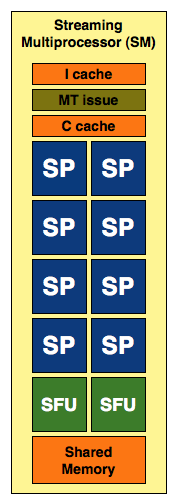
\includegraphics[scale=0.40]{../introduction/assets/SM.png}
\caption{Streaming Multiprocessor}
\label{fig:sm}
\end{wrapfigure}

A CUDA function typically creates many, many threads.
To handle all these, the Fermi architecture has a large number of cores organized into a hierarchy of groups that share different amounts of extra resources.
At its heart lies 16 Streaming Multiprocessors (SMs).

A Streaming Multiprocessor is a collection of tightly coupled Streaming Processor cores (SP) along with some shared accessories.
To enable a large number of cores, NVIDIA makes each of the SP cores simple.
For example, common but difficult functions like sin and reciprocal are delegated to a few separate hardware units within the SM, called Special Function Units (SFU).

In Fermi, each SM contains 32 SP cores. 
Each core is capable of doing both integer and floating point operations.
Their shared accessories include four Special Function units, 16 Load/Store units, and 64KB SRAM for shared memory and shared cache.
A simplified diagram of a smaller SM is shown in Figure \ref{fig:sm}.

\begin{figure}[H]
\centering
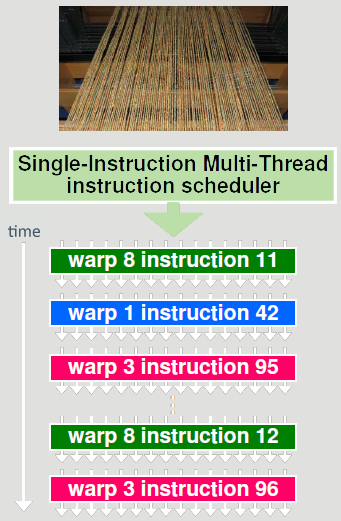
\includegraphics[width=0.4\textwidth]{../introduction/assets/warp.png}
\caption{Warps of 32 threads execute }
\label{fig:simple-nvidia-warps}
\end{figure}

\section{Warps of Threads}

Threads in Fermi are grouped together in logical units of up to 32 threads.
This corresponds to the 32 Streaming Processor cores in a Streaming Multiprocessor.
The 32 threads are collectively called a \emph{warp}. 
Threads in the same warp always execute the same instruction at the same time.
This way, only a single instruction fetch per warp is required for the SM.

Many warps may be active in an SM at any time, and each thread in each warp has its own set of registers within the SM.
This enables fine-grained interleaving of warps without needing expensive context switches with every warp switch. 
A simplified example execution order is shown in figure \ref{fig:simple-nvidia-warps}.
Scheduling warps is difficult, but it is important for filling the pipeline with useful instructions, as discussed in chapter \ref{sec:modern_gpu}

As noted, all instructions in the same warp runs the same instruction.
After a conditional statements, however, different threads of the same warp will likely need to perform different instructions.
This is the concept of thread divergence.
NVIDIA's GPUs support dynamic thread divergence by moving threads between warps as they diverge.

\section{Helpful Inspiration}

The concepts employed in NVIDIA's Fermi architecture and CUDA programming model are, needless to say, effective for parallel calculations.
They have been a source of inspiration for this project.
Most these concepts, like kernels, warps, and easy context switches, will return later in the report.
Although they return in greatly simplified versions, they are helpful for exploiting parallelism.

\end{document}
